

\section{Права доступа}
\textbf{Формулировка задания.}
Создать двух пользователей с следующими правами:
один из пользователей должен иметь право только на просмотр таблицы
\texttt{Cow\_lactation\_diet\_count}, а второй пользователь ---
на просмотр и изменение
таблиц \texttt{Cow}, \texttt{Lactation}, \texttt{Nutrition}.

\subsection{Создание пользователей}

В ходе работы были созданы два пользователя: resultsReader,\\
resultsEditor
(см. листинг \ref{lst:создание_пользователей}).

\begin{lstlisting}[caption={Создание пользователей}, label={lst:создание_пользователей}]
CREATE USER resultsReader WITH PASSWORD '*';
CREATE USER resultsEditor WITH PASSWORD '*';
\end{lstlisting}

В листинге \ref{lst:права_на_бд} представлены SQL-команды,
которые обеспечивают доступ новым пользователям к объектам базы данных.
Первая команда предоставляет обоим пользователям право подключения
к базе данных \texttt{cows\_db}.
Вторая команда предоставляет возможность обоим пользователям
обращаться к объектам, расположенным в схеме public.
Третья команда выдаёт пользователю \texttt{resultsEditor} право на
использование всех последовательностей в схеме public,
что необходимо для создания новых записей в таблицах,
содержащих автоинкрементные поля (SERIAL).

\begin{lstlisting}[caption={Общие права на базу данных}, label={lst:права_на_бд}]
GRANT CONNECT ON DATABASE cows_db TO resultsReader, resultsEditor;
GRANT USAGE ON SCHEMA public TO resultsReader, resultsEditor;
GRANT USAGE ON ALL SEQUENCES IN SCHEMA public TO resultsEditor;
\end{lstlisting}

В листинге \ref{lst:права_на_таблицы} представлены SQL-команды,
с помощью которых новым пользователям были выданы права на чтение или изменение
таблиц. Пользователю resultsReader выдано право только на чтение таблицы
\texttt{Cow\_lactation\_diet\_count}, а пользователю \texttt{resultsEditor} ---
на чтение и изменение таблиц \texttt{Cow}, \texttt{Lactation}, \texttt{Nutrition}.

\begin{lstlisting}[caption={Права на таблицы}, label={lst:права_на_таблицы}]
GRANT SELECT ON Cow_lactation_diet_count TO resultsReader;
GRANT SELECT, INSERT, DELETE, UPDATE ON Cow, Lactation, Nutrition TO resultsEditor;
\end{lstlisting}

В листинге \ref{lst:изм_триг_функ} представлено изменение
триггерных функций. Добавлено \texttt{SECURITY DEFINER}~---
выполнение функции с правами её создателя, а не вызывающего.
Это необходимо для того, чтобы при изменении таблиц пользователем
\texttt{resultsEditor} вызывались триггерные функции,
несмотря на то что текущий пользователь не имеет доступа к таблице\\
\texttt{Cow\_lactation\_diet\_count}, обновляемой триггерами.

\begin{lstlisting}[caption={Изменение триггерных функций}, label={lst:изм_триг_функ}]
ALTER FUNCTION Cow_insert_trigger_function() SECURITY DEFINER;
ALTER FUNCTION Cow_delete_trigger_function() SECURITY DEFINER;
ALTER FUNCTION Nutrition_insert_trigger_function() SECURITY DEFINER;
ALTER FUNCTION Nutrition_delete_trigger_function() SECURITY DEFINER;
ALTER FUNCTION Nutrition_update_trigger_function() SECURITY DEFINER;
ALTER FUNCTION Lactation_insert_trigger_function() SECURITY DEFINER;
ALTER FUNCTION Lactation_delete_trigger_function() SECURITY DEFINER;
ALTER FUNCTION Lactation_update_trigger_function() SECURITY DEFINER;
\end{lstlisting}

\subsection{Результаты работы}

На рисунке \ref{select_editor_err} представлен вывод ошибки при попытке
просмотра таблицы \texttt{Cow\_lactation\_diet\_count} пользователем
\texttt{resultsEditor}.
\begin{figure}[H]
    \centering
    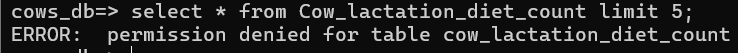
\includegraphics[width=\linewidth]{images/select_editor_err.png}
    \caption{Ошибка доступа пользователя \texttt{resultsEditor} к таблице \texttt{Cow\_lactation\_diet\_count}}
    \label{select_editor_err}
\end{figure}

На рисунке \ref{select_editor_ok} представлен вывод строк из таблиц
\texttt{Cow}, \texttt{Lactation}, \texttt{Nutrition} после запросов
\texttt{SELECT} пользователем \texttt{resultsEditor}.
\begin{figure}[H]
    \centering
    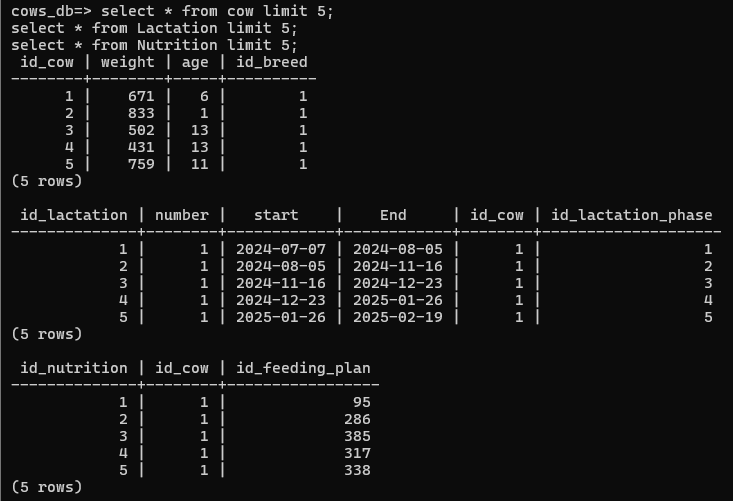
\includegraphics[width=\linewidth]{images/select_editor_ok.png}
    \caption{Успешный просмотр таблиц \texttt{Cow}, \texttt{Lactation}, \texttt{Nutrition} пользователем \texttt{resultsEditor}}
    \label{select_editor_ok}
\end{figure}

На рисунке \ref{select_reader_ok} представлен вывод строк из таблицы
\texttt{Cow\_lactation\_diet\_count} после запроса \texttt{SELECT}
пользователем \texttt{resultsReader}.
\begin{figure}[H]
    \centering
    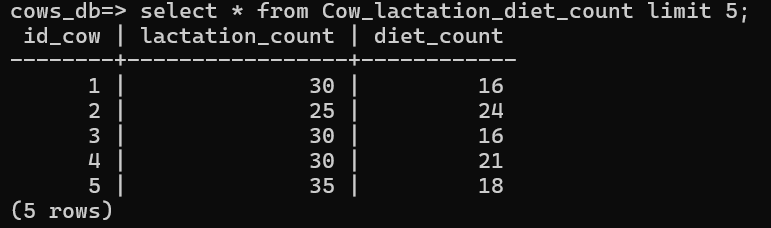
\includegraphics[width=0.8\linewidth]{images/select_reader_ok.png}
    \caption{Успешный просмотр таблицы \texttt{Cow\_lactation\_diet\_count} пользователем \texttt{resultsReader}}
    \label{select_reader_ok}
\end{figure}

На рисунке \ref{select_reader_err} представлен вывод ошибки при
попытке просмотра таблицы \texttt{Cow}
пользователем \texttt{resultsReader}.
\begin{figure}[H]
    \centering
    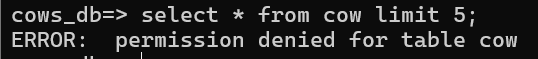
\includegraphics[width=0.7\linewidth]{images/select_reader_err.png}
    \caption{Ошибка доступа пользователя \texttt{resultsReader} к таблице \texttt{Cow}}
    \label{select_reader_err}
\end{figure}

На рисунке \ref{edit_cow} представлен пример добавления записи в таблицу
\texttt{Cow} пользователем \texttt{resultsEditor}, а также изменение и удаление
этой записи.
\begin{figure}[H]
    \centering
    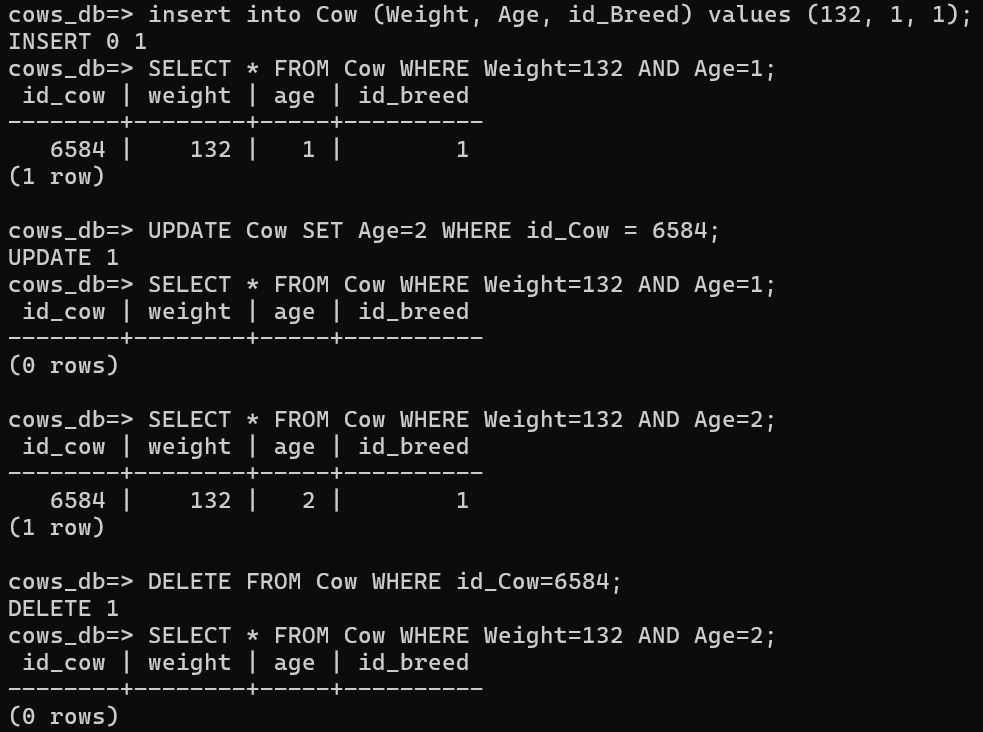
\includegraphics[width=0.9\linewidth]{images/edit_cow.png}
    \caption{Операции \texttt{INSERT}, \texttt{UPDATE} и \texttt{DELETE} в таблице \texttt{Cow} пользователем \texttt{resultsEditor}}
    \label{edit_cow}
\end{figure}

На рисунке \ref{after_insert} представлен пример добавления записи
в таблицу \texttt{Cow} пользователем \texttt{resultsEditor}
и автоматическое добавление записи в таблицу \texttt{Cow\_lactation\_diet\_count}.
\begin{figure}[H]
    \centering
    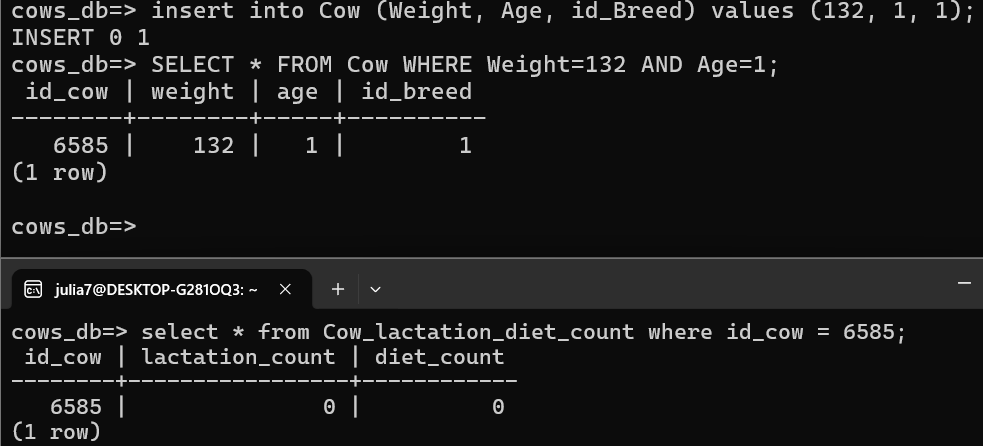
\includegraphics[width=0.9\linewidth]{images/after_insert.png}
    \caption{Автоматическое обновление таблицы триггером при добавлении записи в таблицу \texttt{Cow}}
    \label{after_insert}
\end{figure}

В таблице \ref{tab:проверка_прав} приведены сравнительные результаты
проверки прав доступа пользователей.

\begin{table}[h!]
\centering
\caption{Результаты проверки прав доступа пользователей}
\label{tab:проверка_прав}
\begin{tabular}{|c|c|c|}
\hline
\textnumero & \textbf{resultsReader} & \textbf{resultsEditor} \\
\hline
\multicolumn{3}{|c|}{\texttt{SELECT * FROM Cow\_lactation\_diet\_count LIMIT 5;}} \\
\hline
1 & Результат запроса & Ошибка доступа \\
\hline
\multicolumn{3}{|c|}{\texttt{SELECT * FROM Cow LIMIT 5;}} \\
\hline
2 & Ошибка доступа & Результат запроса \\
\hline
\multicolumn{3}{|c|}{\texttt{INSERT INTO Cow (Weight, Age, id\_Breed) VALUES (160, 2, 3);}} \\
\hline
3 & Ошибка доступа & Выполненный запрос \\
\hline
\multicolumn{3}{|c|}{\texttt{UPDATE Cow SET Age = 2 WHERE id\_Cow = 6584;}} \\
\hline
4 & Ошибка доступа & Выполненный запрос \\
\hline
\multicolumn{3}{|c|}{\texttt{DELETE FROM Cow WHERE id\_Cow = 6584;}} \\
\hline
5 & Ошибка доступа & Выполненный запрос \\
\hline
\multicolumn{3}{|c|}{\texttt{SELECT * FROM Lactation LIMIT 5;}} \\
\hline
6 & Ошибка доступа & Результат запроса \\
\hline
\multicolumn{3}{|c|}{\texttt{SELECT * FROM Breed LIMIT 5;}} \\
\hline
7 & Ошибка доступа & Ошибка доступа \\
\hline
\end{tabular}
\end{table}